% Options for packages loaded elsewhere
\PassOptionsToPackage{unicode}{hyperref}
\PassOptionsToPackage{hyphens}{url}
%
\documentclass[
]{article}
\usepackage{lmodern}
\usepackage{amssymb,amsmath}
\usepackage{ifxetex,ifluatex}
\ifnum 0\ifxetex 1\fi\ifluatex 1\fi=0 % if pdftex
  \usepackage[T1]{fontenc}
  \usepackage[utf8]{inputenc}
  \usepackage{textcomp} % provide euro and other symbols
\else % if luatex or xetex
  \usepackage{unicode-math}
  \defaultfontfeatures{Scale=MatchLowercase}
  \defaultfontfeatures[\rmfamily]{Ligatures=TeX,Scale=1}
\fi
% Use upquote if available, for straight quotes in verbatim environments
\IfFileExists{upquote.sty}{\usepackage{upquote}}{}
\IfFileExists{microtype.sty}{% use microtype if available
  \usepackage[]{microtype}
  \UseMicrotypeSet[protrusion]{basicmath} % disable protrusion for tt fonts
}{}
\makeatletter
\@ifundefined{KOMAClassName}{% if non-KOMA class
  \IfFileExists{parskip.sty}{%
    \usepackage{parskip}
  }{% else
    \setlength{\parindent}{0pt}
    \setlength{\parskip}{6pt plus 2pt minus 1pt}}
}{% if KOMA class
  \KOMAoptions{parskip=half}}
\makeatother
\usepackage{xcolor}
\IfFileExists{xurl.sty}{\usepackage{xurl}}{} % add URL line breaks if available
\IfFileExists{bookmark.sty}{\usepackage{bookmark}}{\usepackage{hyperref}}
\hypersetup{
  pdftitle={Stats 504 Homework 2},
  hidelinks,
  pdfcreator={LaTeX via pandoc}}
\urlstyle{same} % disable monospaced font for URLs
\usepackage[margin=1in]{geometry}
\usepackage{color}
\usepackage{fancyvrb}
\newcommand{\VerbBar}{|}
\newcommand{\VERB}{\Verb[commandchars=\\\{\}]}
\DefineVerbatimEnvironment{Highlighting}{Verbatim}{commandchars=\\\{\}}
% Add ',fontsize=\small' for more characters per line
\usepackage{framed}
\definecolor{shadecolor}{RGB}{248,248,248}
\newenvironment{Shaded}{\begin{snugshade}}{\end{snugshade}}
\newcommand{\AlertTok}[1]{\textcolor[rgb]{0.94,0.16,0.16}{#1}}
\newcommand{\AnnotationTok}[1]{\textcolor[rgb]{0.56,0.35,0.01}{\textbf{\textit{#1}}}}
\newcommand{\AttributeTok}[1]{\textcolor[rgb]{0.77,0.63,0.00}{#1}}
\newcommand{\BaseNTok}[1]{\textcolor[rgb]{0.00,0.00,0.81}{#1}}
\newcommand{\BuiltInTok}[1]{#1}
\newcommand{\CharTok}[1]{\textcolor[rgb]{0.31,0.60,0.02}{#1}}
\newcommand{\CommentTok}[1]{\textcolor[rgb]{0.56,0.35,0.01}{\textit{#1}}}
\newcommand{\CommentVarTok}[1]{\textcolor[rgb]{0.56,0.35,0.01}{\textbf{\textit{#1}}}}
\newcommand{\ConstantTok}[1]{\textcolor[rgb]{0.00,0.00,0.00}{#1}}
\newcommand{\ControlFlowTok}[1]{\textcolor[rgb]{0.13,0.29,0.53}{\textbf{#1}}}
\newcommand{\DataTypeTok}[1]{\textcolor[rgb]{0.13,0.29,0.53}{#1}}
\newcommand{\DecValTok}[1]{\textcolor[rgb]{0.00,0.00,0.81}{#1}}
\newcommand{\DocumentationTok}[1]{\textcolor[rgb]{0.56,0.35,0.01}{\textbf{\textit{#1}}}}
\newcommand{\ErrorTok}[1]{\textcolor[rgb]{0.64,0.00,0.00}{\textbf{#1}}}
\newcommand{\ExtensionTok}[1]{#1}
\newcommand{\FloatTok}[1]{\textcolor[rgb]{0.00,0.00,0.81}{#1}}
\newcommand{\FunctionTok}[1]{\textcolor[rgb]{0.00,0.00,0.00}{#1}}
\newcommand{\ImportTok}[1]{#1}
\newcommand{\InformationTok}[1]{\textcolor[rgb]{0.56,0.35,0.01}{\textbf{\textit{#1}}}}
\newcommand{\KeywordTok}[1]{\textcolor[rgb]{0.13,0.29,0.53}{\textbf{#1}}}
\newcommand{\NormalTok}[1]{#1}
\newcommand{\OperatorTok}[1]{\textcolor[rgb]{0.81,0.36,0.00}{\textbf{#1}}}
\newcommand{\OtherTok}[1]{\textcolor[rgb]{0.56,0.35,0.01}{#1}}
\newcommand{\PreprocessorTok}[1]{\textcolor[rgb]{0.56,0.35,0.01}{\textit{#1}}}
\newcommand{\RegionMarkerTok}[1]{#1}
\newcommand{\SpecialCharTok}[1]{\textcolor[rgb]{0.00,0.00,0.00}{#1}}
\newcommand{\SpecialStringTok}[1]{\textcolor[rgb]{0.31,0.60,0.02}{#1}}
\newcommand{\StringTok}[1]{\textcolor[rgb]{0.31,0.60,0.02}{#1}}
\newcommand{\VariableTok}[1]{\textcolor[rgb]{0.00,0.00,0.00}{#1}}
\newcommand{\VerbatimStringTok}[1]{\textcolor[rgb]{0.31,0.60,0.02}{#1}}
\newcommand{\WarningTok}[1]{\textcolor[rgb]{0.56,0.35,0.01}{\textbf{\textit{#1}}}}
\usepackage{longtable,booktabs}
% Correct order of tables after \paragraph or \subparagraph
\usepackage{etoolbox}
\makeatletter
\patchcmd\longtable{\par}{\if@noskipsec\mbox{}\fi\par}{}{}
\makeatother
% Allow footnotes in longtable head/foot
\IfFileExists{footnotehyper.sty}{\usepackage{footnotehyper}}{\usepackage{footnote}}
\makesavenoteenv{longtable}
\usepackage{graphicx,grffile}
\makeatletter
\def\maxwidth{\ifdim\Gin@nat@width>\linewidth\linewidth\else\Gin@nat@width\fi}
\def\maxheight{\ifdim\Gin@nat@height>\textheight\textheight\else\Gin@nat@height\fi}
\makeatother
% Scale images if necessary, so that they will not overflow the page
% margins by default, and it is still possible to overwrite the defaults
% using explicit options in \includegraphics[width, height, ...]{}
\setkeys{Gin}{width=\maxwidth,height=\maxheight,keepaspectratio}
% Set default figure placement to htbp
\makeatletter
\def\fps@figure{htbp}
\makeatother
\setlength{\emergencystretch}{3em} % prevent overfull lines
\providecommand{\tightlist}{%
  \setlength{\itemsep}{0pt}\setlength{\parskip}{0pt}}
\setcounter{secnumdepth}{5}

\title{Stats 504 Homework 2}
\author{}
\date{\vspace{-2.5em}October 10, 2021}

\begin{document}
\maketitle

\hypertarget{introduction}{%
\section{Introduction}\label{introduction}}

Diabetic Retinopathy is a retinal disorder in diabetes patients which
can cause blindness. There exists two laser treatments, argon/xenon,
that can help delay diabetic retinopathy. In this analysis, we plan to
determine the efficacy and quantify the improvement of each laser
treatment on visual acuity. Moreover, we want to explain the influence
of age and clinical risk of diabetic retinopathy on visual acuity.

\hypertarget{method}{%
\section{Method}\label{method}}

In this analysis, our target is to figure out the efficacy of two laser
treatments and analyze the effect of age and clinical risk. We first use
Kaplan-Meier Estimator to plot the survival curve curve and test if
there is a difference between the survival curves. And then we use Cox
Proportional Hazards Model to fit the data and quantify the relationship
between the predictors and hazards functions. We also noticed that in
this dataset, every two rows can be treated as a cluster, since they are
just left and right eyes of one patient. There exists some associations
between observations. In order to address this issue, we consider the
frailty model, we just include a frailty term \texttt{frailty(id)} in
our Cox PH model.

\hypertarget{result}{%
\section{Result}\label{result}}

The whole dataset contains 197 patients and 394 observations. It has
totally 10 columns and does not have any missing value. We defined a new
variable \texttt{survobj} as our response variable in this analysis,
which is a survival object and combines the information of
\texttt{futime} and \texttt{status}. We also created a new variable
\texttt{treatment} which encodes the \texttt{laser} to `control' when
\texttt{trt} equals 0. In this dataset, \texttt{age} and \texttt{type}
contain redundant information, we just use \texttt{type} in Kaplan-Meier
Estimator and \texttt{age} in Cox Proportional Hazards Model. Since
there is no casual relationship between other predictors in this
dataset, we also include \texttt{eye} and \texttt{risk} in our model.

\hypertarget{kaplan-meier-estimation}{%
\subsection{Kaplan-Meier Estimation}\label{kaplan-meier-estimation}}

The following figure shows survival curve against \texttt{treatment},
\texttt{type}, \texttt{eye} and \texttt{risk}. Through the figure we can
see that in the plot against \texttt{treatment} and \texttt{risk}, the
difference between curves is relatively larger than the rest two plots.
Moreover, the difference increases as time increases. As time goes by,
the survival curve of control group and high clinical risk group
drcreases faster than the others.

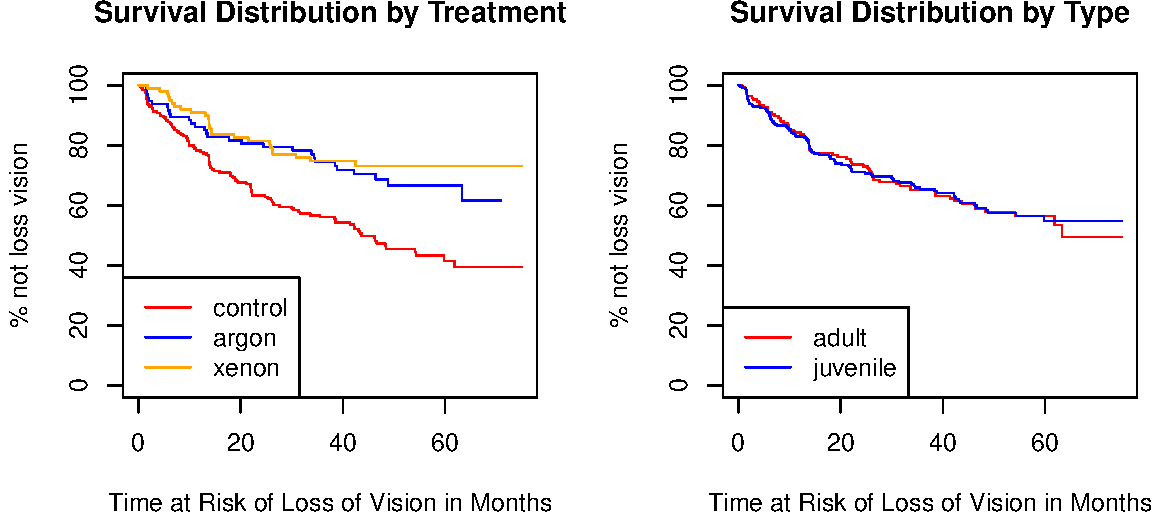
\includegraphics{stats504_hw2_files/figure-latex/unnamed-chunk-2-1.pdf}
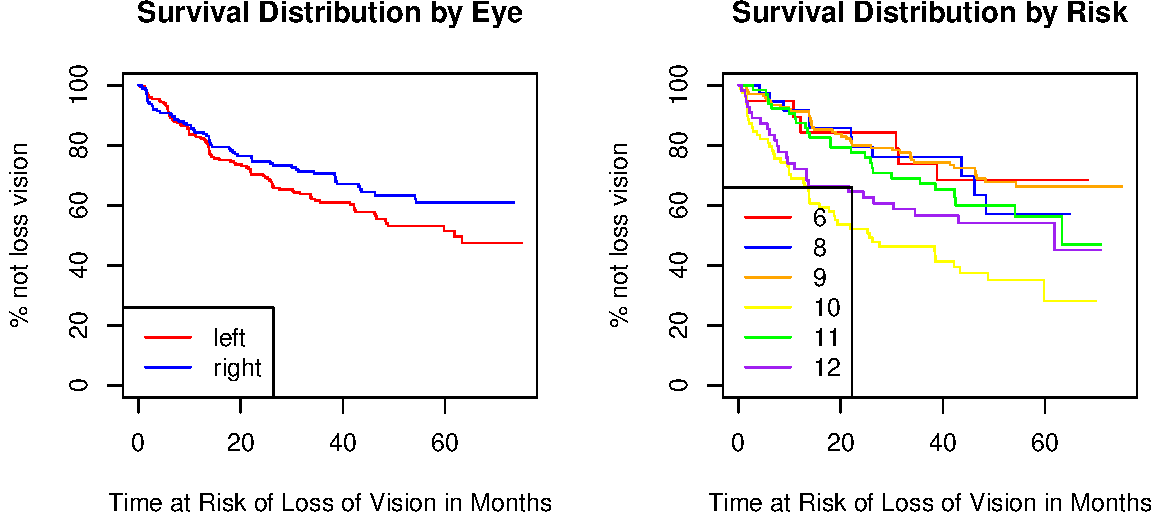
\includegraphics{stats504_hw2_files/figure-latex/unnamed-chunk-2-2.pdf}

We also conduct a log-rank test to test whether there is a true
difference between survival curves. The hypothesis of the log-rank test
as follows.\\
\(H_0\) : There is no difference in the Kaplan-Meier survival curve
between different groups.\\
\(H_1\) : There is a difference in the Kaplan-Meier survival curve
between different groups.\\
The result is shown in the following table. We can see that for the
difference between \texttt{treatment} group and \texttt{risk} group they
are statistical significant, and we do not have enough statistical
evidence to conclude the difference between \texttt{eye} group and
\texttt{type} group.

\begin{longtable}[]{@{}lll@{}}
\caption{The Log-rank Test}\tabularnewline
\toprule
Variable & Chisq2 & P-value\tabularnewline
\midrule
\endfirsthead
\toprule
Variable & Chisq2 & P-value\tabularnewline
\midrule
\endhead
Treatment & 22.666 & 2e-06\tabularnewline
Type & 0.017 & 0.894859\tabularnewline
Eye & 2.788 & 0.094968\tabularnewline
Risk & 32.962 & 0\tabularnewline
\bottomrule
\end{longtable}

\hypertarget{cox-proportional-hazards-model}{%
\subsection{Cox Proportional Hazards
Model}\label{cox-proportional-hazards-model}}

In this section, we first conduct the classical Cox Proportional Hazards
Model using \texttt{survobj} as response and \texttt{eye}, \texttt{age},
\texttt{risk}, \texttt{treatment} as predictors. Then we conduct
hypotheses to test the proportional hazards assumptions for the Cox PH
model. The result indicates that the proportional assumption of Cox PH
model is satisfied quite well here.

\begin{longtable}[]{@{}lrrrrrrr@{}}
\caption{The Cox Proportion Hazard Model}\tabularnewline
\toprule
& coef & z & Pr(\textgreater\textbar z\textbar) & exp(coef) & exp(-coef)
& lower .95 & upper .95\tabularnewline
\midrule
\endfirsthead
\toprule
& coef & z & Pr(\textgreater\textbar z\textbar) & exp(coef) & exp(-coef)
& lower .95 & upper .95\tabularnewline
\midrule
\endhead
eyeright & -0.2225 & -1.3281 & 0.1841 & 0.8005 & 1.2492 & 0.5765 &
1.1116\tabularnewline
age & 0.0059 & 1.0673 & 0.2858 & 1.0059 & 0.9941 & 0.9951 &
1.0168\tabularnewline
risk & 0.1426 & 2.5341 & 0.0113 & 1.1533 & 0.8671 & 1.0328 &
1.2877\tabularnewline
treatmentargon & -0.6918 & -3.2730 & 0.0011 & 0.5007 & 1.9974 & 0.3308 &
0.7576\tabularnewline
treatmentxenon & -0.8762 & -3.9054 & 0.0001 & 0.4163 & 2.4019 & 0.2682 &
0.6463\tabularnewline
\bottomrule
\end{longtable}

\begin{longtable}[]{@{}lrrr@{}}
\caption{Proportional Hazards Assumption Test}\tabularnewline
\toprule
& chisq & df & p\tabularnewline
\midrule
\endfirsthead
\toprule
& chisq & df & p\tabularnewline
\midrule
\endhead
eye & 0.8010425 & 1 & 0.3707819\tabularnewline
age & 0.3635736 & 1 & 0.5465282\tabularnewline
risk & 1.6921822 & 1 & 0.1933136\tabularnewline
treatment & 0.5946964 & 2 & 0.7427853\tabularnewline
GLOBAL & 3.7861712 & 5 & 0.5805942\tabularnewline
\bottomrule
\end{longtable}

To address the association between the left and right eyes of one
person, we conducted a Frailty Cox PH model, which adds a simple random
effects term to allow intra-person correlation in one patient.

\begin{longtable}[]{@{}llllllll@{}}
\caption{The Frailty Cox Proportional Hazards Model}\tabularnewline
\toprule
& coef & Chisq & p & exp(coef) & exp(-coef) & lower .95 & upper
.95\tabularnewline
\midrule
\endfirsthead
\toprule
& coef & Chisq & p & exp(coef) & exp(-coef) & lower .95 & upper
.95\tabularnewline
\midrule
\endhead
eyeright & -0.3127 & 2.0069 & 0.1566 & 0.7315 & 1.3671 & 0.4746 &
1.1274\tabularnewline
age & 0.0075 & 1.0279 & 0.3107 & 1.0075 & 0.9926 & 0.9931 &
1.0221\tabularnewline
risk & 0.1642 & 5.6454 & 0.0175 & 1.1785 & 0.8486 & 1.0292 &
1.3494\tabularnewline
treatmentargon & -0.8504 & 14.1398 & 2e-04 & 0.4273 & 2.3405 & 0.2743 &
0.6656\tabularnewline
treatmentxenon & -0.9553 & 16.5165 & 0 & 0.3847 & 2.5995 & 0.2427 &
0.6098\tabularnewline
frailty(id) & NA & 104.0195 & 0.0235 & & & &\tabularnewline
\bottomrule
\end{longtable}

After Comparing these two models, we can see that the coefficients and
significant tests are quite similar. \texttt{Argon} treatment,
\texttt{Xenon} treatment and \texttt{Risk} are statistically significant
in both models, and rest predictors are not. Here we use Frailty Cox PH
model to quantify the efficacy of two laser treatments. The exponential
coefficient of \texttt{Argon} treatment is 0.4273 (95\% {[}0.2743,
0.6656{]}) and the exponential coefficient of \texttt{Xenon} treatment
is 0.3847 (95\% {[}0.2427, 0.6098{]}). Comparing with the control group,
\texttt{Argon} treatment can decrease the risk of visual loss to 42.73\%
(95\% {[}27.43\%, 66.56\%{]}) and \texttt{Xenon} treatment can decrease
the risk of visual loss to 38.47\% (95\% {[}24.27\%, 60.98\%{]}). The
\texttt{Xenon} treatment can provide relatively better treatment effect.
AS for the effect of \texttt{age} and \texttt{risk}, since \texttt{age}
is not statistically significant we can not conclude any effect of
\texttt{age} on the risk of visual loss. The exponential coefficient of
\texttt{risk} treatment is 1.1785 (95\% {[}1.0292, 1.3494{]}), which
indicates that 1-unit increase in clinical risk, the risk of visual loss
will also increase 17.85\% (95\% CI {[}2.92\%, 34.94\%{]}).

\hypertarget{conclusion}{%
\section{Conclusion}\label{conclusion}}

This analysis is aimed to quantify the efficacy of \texttt{Argon} and
\texttt{Xenon} treatments, and explains the effect of \texttt{age} and
\texttt{clinical\ risk} on the risk of visual loss. The Frailty Cox
Proportional Hazards Model seems characterize the hazards function quite
well in this question. In conclusion, both \texttt{Argon} and
\texttt{Xenon} treatments certainly have significant positive treatment
effect on visual acuity, \texttt{clinical\ risk} have negative influence
on visual acuity, and we do not have enough evidence to show the effect
of \texttt{age} on visual acuity.

\hypertarget{appendix}{%
\section{Appendix}\label{appendix}}

Source code of this report can be found
\href{https://github.com/ZhihaoXu/Stats504/blob/main/Assignment/assignment_2/stats504_hw2.Rmd}{\emph{here}}.

\begin{Shaded}
\begin{Highlighting}[]
\KeywordTok{library}\NormalTok{(survival)}
\KeywordTok{library}\NormalTok{(tidyverse)}
\KeywordTok{library}\NormalTok{(Hmisc)}

\NormalTok{df =}\StringTok{ }\KeywordTok{read.delim}\NormalTok{(}\StringTok{'diabeticVision.csv'}\NormalTok{, }\DataTypeTok{sep=}\StringTok{','}\NormalTok{)}
\NormalTok{df =}\StringTok{ }\NormalTok{df }\OperatorTok
\StringTok{  }\KeywordTok{mutate}\NormalTok{(}
    \DataTypeTok{tr_eye =} \KeywordTok{ifelse}\NormalTok{(trt}\OperatorTok{==}\DecValTok{1}\NormalTok{, eye, }\KeywordTok{ifelse}\NormalTok{(eye}\OperatorTok{==}\StringTok{'left'}\NormalTok{, }\StringTok{'right'}\NormalTok{, }\StringTok{'left'}\NormalTok{)),}
    \DataTypeTok{treatment =} \KeywordTok{ifelse}\NormalTok{(trt}\OperatorTok{==}\DecValTok{1}\NormalTok{, laser, }\StringTok{'control'}\NormalTok{)}
\NormalTok{  )}
\NormalTok{df}\OperatorTok{$}\NormalTok{treatment =}\StringTok{  }\KeywordTok{relevel}\NormalTok{(}\KeywordTok{as.factor}\NormalTok{(df}\OperatorTok{$}\NormalTok{treatment), }\DataTypeTok{ref=}\StringTok{'control'}\NormalTok{)}

\NormalTok{survobj =}\StringTok{ }\KeywordTok{with}\NormalTok{(df, }\KeywordTok{Surv}\NormalTok{(futime, status))}

\NormalTok{plot_survfit =}\StringTok{ }\ControlFlowTok{function}\NormalTok{(var)\{}
\NormalTok{  fitr <-}\StringTok{ }\KeywordTok{survfit}\NormalTok{(}\KeywordTok{as.formula}\NormalTok{(}\KeywordTok{paste0}\NormalTok{(}\StringTok{'survobj~'}\NormalTok{, var)), }\DataTypeTok{data=}\NormalTok{df)}
  \KeywordTok{plot}\NormalTok{(fitr, }\DataTypeTok{xlab=}\StringTok{"Time at Risk of Loss of Vision in Months"}\NormalTok{,}
   \DataTypeTok{ylab=}\StringTok{"% not loss vision"}\NormalTok{, }\DataTypeTok{yscale=}\DecValTok{100}\NormalTok{,}
   \DataTypeTok{main=}\KeywordTok{paste}\NormalTok{(}\StringTok{"Survival Distribution by"}\NormalTok{, }\KeywordTok{capitalize}\NormalTok{(var)),}
   \DataTypeTok{col =} \KeywordTok{c}\NormalTok{(}\StringTok{'red'}\NormalTok{, }\StringTok{'blue'}\NormalTok{, }\StringTok{'orange'}\NormalTok{, }\StringTok{'yellow'}\NormalTok{, }\StringTok{'green'}\NormalTok{, }\StringTok{'purple'}\NormalTok{))}
  \KeywordTok{legend}\NormalTok{(}\StringTok{'bottomleft'}\NormalTok{, }\DataTypeTok{legend=}\KeywordTok{levels}\NormalTok{(}\KeywordTok{as.factor}\NormalTok{(df[,var])), }
         \DataTypeTok{col =} \KeywordTok{c}\NormalTok{(}\StringTok{'red'}\NormalTok{, }\StringTok{'blue'}\NormalTok{, }\StringTok{'orange'}\NormalTok{, }\StringTok{'yellow'}\NormalTok{, }\StringTok{'green'}\NormalTok{, }\StringTok{'purple'}\NormalTok{), }\DataTypeTok{lty=}\DecValTok{1}\NormalTok{)}
\NormalTok{\}}
\KeywordTok{par}\NormalTok{(}\DataTypeTok{mfrow=}\KeywordTok{c}\NormalTok{(}\DecValTok{1}\NormalTok{,}\DecValTok{2}\NormalTok{))}
\KeywordTok{plot_survfit}\NormalTok{(}\StringTok{'treatment'}\NormalTok{)}
\KeywordTok{plot_survfit}\NormalTok{(}\StringTok{'type'}\NormalTok{)}
\end{Highlighting}
\end{Shaded}

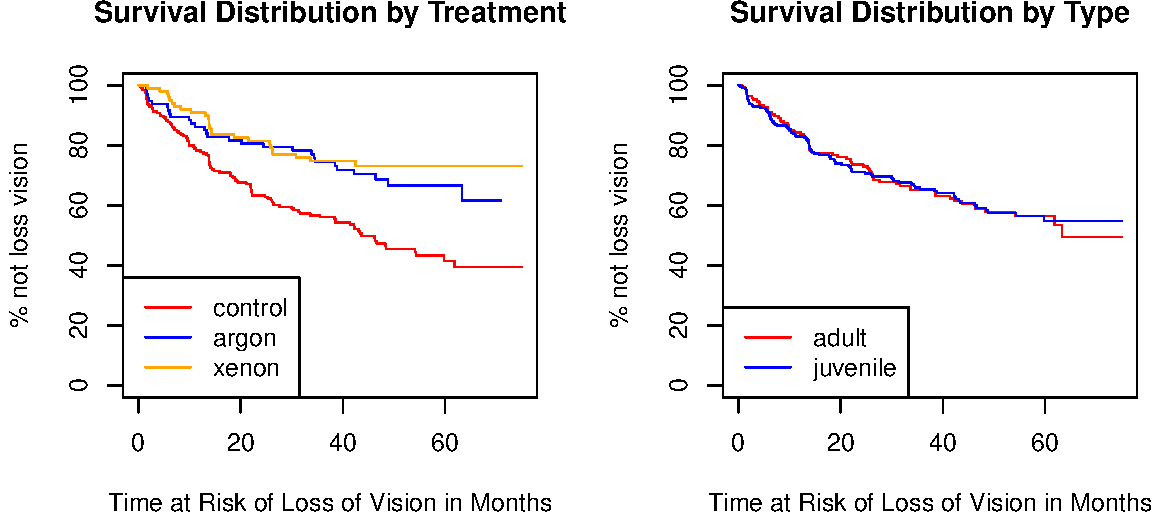
\includegraphics{stats504_hw2_files/figure-latex/unnamed-chunk-6-1.pdf}

\begin{Shaded}
\begin{Highlighting}[]
\KeywordTok{plot_survfit}\NormalTok{(}\StringTok{'eye'}\NormalTok{)}
\KeywordTok{plot_survfit}\NormalTok{(}\StringTok{'risk'}\NormalTok{)}
\end{Highlighting}
\end{Shaded}

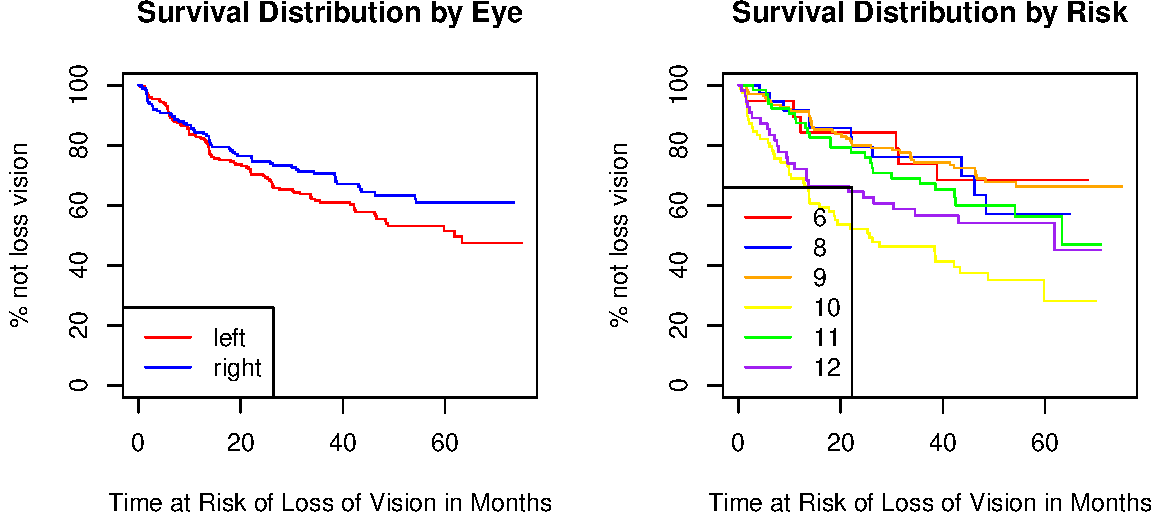
\includegraphics{stats504_hw2_files/figure-latex/unnamed-chunk-6-2.pdf}

\begin{Shaded}
\begin{Highlighting}[]
\NormalTok{dif_res =}\StringTok{ }\KeywordTok{rbind}\NormalTok{(}
  \KeywordTok{c}\NormalTok{(}\StringTok{'Treatment'}\NormalTok{, }\KeywordTok{survdiff}\NormalTok{(survobj}\OperatorTok{~}\NormalTok{treatment, }\DataTypeTok{data=}\NormalTok{df)}\OperatorTok{$}\NormalTok{chisq, }\DecValTok{1} \OperatorTok{-}\StringTok{ }\KeywordTok{pchisq}\NormalTok{(}\KeywordTok{survdiff}\NormalTok{(survobj}\OperatorTok{~}\NormalTok{treatment, }\DataTypeTok{data=}\NormalTok{df)}\OperatorTok{$}\NormalTok{chisq, }\DataTypeTok{df=}\DecValTok{1}\NormalTok{)), }
  \KeywordTok{c}\NormalTok{(}\StringTok{'Type'}\NormalTok{, }\KeywordTok{survdiff}\NormalTok{(survobj}\OperatorTok{~}\NormalTok{type, }\DataTypeTok{data=}\NormalTok{df)}\OperatorTok{$}\NormalTok{chisq, }\DecValTok{1} \OperatorTok{-}\StringTok{ }\KeywordTok{pchisq}\NormalTok{(}\KeywordTok{survdiff}\NormalTok{(survobj}\OperatorTok{~}\NormalTok{type, }\DataTypeTok{data=}\NormalTok{df)}\OperatorTok{$}\NormalTok{chisq, }\DataTypeTok{df=}\DecValTok{1}\NormalTok{)),}
  \KeywordTok{c}\NormalTok{(}\StringTok{'Eye'}\NormalTok{, }\KeywordTok{survdiff}\NormalTok{(survobj}\OperatorTok{~}\NormalTok{eye, }\DataTypeTok{data=}\NormalTok{df)}\OperatorTok{$}\NormalTok{chisq, }\DecValTok{1} \OperatorTok{-}\StringTok{ }\KeywordTok{pchisq}\NormalTok{(}\KeywordTok{survdiff}\NormalTok{(survobj}\OperatorTok{~}\NormalTok{eye, }\DataTypeTok{data=}\NormalTok{df)}\OperatorTok{$}\NormalTok{chisq, }\DataTypeTok{df=}\DecValTok{1}\NormalTok{)),}
  \KeywordTok{c}\NormalTok{(}\StringTok{'Risk'}\NormalTok{, }\KeywordTok{survdiff}\NormalTok{(survobj}\OperatorTok{~}\NormalTok{risk, }\DataTypeTok{data=}\NormalTok{df)}\OperatorTok{$}\NormalTok{chisq, }\DecValTok{1} \OperatorTok{-}\StringTok{ }\KeywordTok{pchisq}\NormalTok{(}\KeywordTok{survdiff}\NormalTok{(survobj}\OperatorTok{~}\NormalTok{risk, }\DataTypeTok{data=}\NormalTok{df)}\OperatorTok{$}\NormalTok{chisq, }\DataTypeTok{df=}\DecValTok{1}\NormalTok{)))}
\NormalTok{dif_res[,}\KeywordTok{c}\NormalTok{(}\DecValTok{2}\NormalTok{)] =}\StringTok{ }\KeywordTok{round}\NormalTok{(}\KeywordTok{as.numeric}\NormalTok{(dif_res[,}\KeywordTok{c}\NormalTok{(}\DecValTok{2}\NormalTok{)]), }\DecValTok{3}\NormalTok{)}
\NormalTok{dif_res[,}\KeywordTok{c}\NormalTok{(}\DecValTok{3}\NormalTok{)] =}\StringTok{ }\KeywordTok{round}\NormalTok{(}\KeywordTok{as.numeric}\NormalTok{(dif_res[,}\KeywordTok{c}\NormalTok{(}\DecValTok{3}\NormalTok{)]), }\DecValTok{6}\NormalTok{)}
\NormalTok{dif_res }\OperatorTok\StringTok{ }\NormalTok{knitr}\OperatorTok{::}\KeywordTok{kable}\NormalTok{(}\DataTypeTok{col.names =} \KeywordTok{c}\NormalTok{(}\StringTok{'Variable'}\NormalTok{, }\StringTok{'Chisq2'}\NormalTok{, }\StringTok{'P-value'}\NormalTok{), }\DataTypeTok{caption =} \StringTok{'The Log-rank Test'}\NormalTok{)}
\end{Highlighting}
\end{Shaded}

\begin{longtable}[]{@{}lll@{}}
\caption{The Log-rank Test}\tabularnewline
\toprule
Variable & Chisq2 & P-value\tabularnewline
\midrule
\endfirsthead
\toprule
Variable & Chisq2 & P-value\tabularnewline
\midrule
\endhead
Treatment & 22.666 & 2e-06\tabularnewline
Type & 0.017 & 0.894859\tabularnewline
Eye & 2.788 & 0.094968\tabularnewline
Risk & 32.962 & 0\tabularnewline
\bottomrule
\end{longtable}

\begin{Shaded}
\begin{Highlighting}[]
\NormalTok{cox_model =}\StringTok{ }\KeywordTok{summary}\NormalTok{(}\KeywordTok{coxph}\NormalTok{(survobj}\OperatorTok{~}\NormalTok{eye}\OperatorTok{+}\NormalTok{age}\OperatorTok{+}\NormalTok{risk}\OperatorTok{+}\NormalTok{treatment, }\DataTypeTok{data=}\NormalTok{df))}
\KeywordTok{cbind}\NormalTok{(}\KeywordTok{round}\NormalTok{(cox_model}\OperatorTok{$}\NormalTok{coefficients[,}\KeywordTok{c}\NormalTok{(}\DecValTok{1}\NormalTok{,}\DecValTok{4}\NormalTok{,}\DecValTok{5}\NormalTok{)], }\DecValTok{4}\NormalTok{), }\KeywordTok{round}\NormalTok{(cox_model}\OperatorTok{$}\NormalTok{conf.int,}\DecValTok{4}\NormalTok{))}\OperatorTok
\StringTok{  }\NormalTok{knitr}\OperatorTok{::}\KeywordTok{kable}\NormalTok{(}\DataTypeTok{caption =} \StringTok{'The Cox Proportion Hazard Model'}\NormalTok{)}
\end{Highlighting}
\end{Shaded}

\begin{longtable}[]{@{}lrrrrrrr@{}}
\caption{The Cox Proportion Hazard Model}\tabularnewline
\toprule
& coef & z & Pr(\textgreater\textbar z\textbar) & exp(coef) & exp(-coef)
& lower .95 & upper .95\tabularnewline
\midrule
\endfirsthead
\toprule
& coef & z & Pr(\textgreater\textbar z\textbar) & exp(coef) & exp(-coef)
& lower .95 & upper .95\tabularnewline
\midrule
\endhead
eyeright & -0.2225 & -1.3281 & 0.1841 & 0.8005 & 1.2492 & 0.5765 &
1.1116\tabularnewline
age & 0.0059 & 1.0673 & 0.2858 & 1.0059 & 0.9941 & 0.9951 &
1.0168\tabularnewline
risk & 0.1426 & 2.5341 & 0.0113 & 1.1533 & 0.8671 & 1.0328 &
1.2877\tabularnewline
treatmentargon & -0.6918 & -3.2730 & 0.0011 & 0.5007 & 1.9974 & 0.3308 &
0.7576\tabularnewline
treatmentxenon & -0.8762 & -3.9054 & 0.0001 & 0.4163 & 2.4019 & 0.2682 &
0.6463\tabularnewline
\bottomrule
\end{longtable}

\begin{Shaded}
\begin{Highlighting}[]
\NormalTok{gof =}\StringTok{ }\KeywordTok{cox.zph}\NormalTok{(}\KeywordTok{coxph}\NormalTok{(survobj}\OperatorTok{~}\NormalTok{eye}\OperatorTok{+}\NormalTok{age}\OperatorTok{+}\NormalTok{risk}\OperatorTok{+}\NormalTok{treatment, }\DataTypeTok{data=}\NormalTok{df)) }
\NormalTok{gof}\OperatorTok{$}\NormalTok{table }\OperatorTok\StringTok{ }\NormalTok{knitr}\OperatorTok{::}\KeywordTok{kable}\NormalTok{(}\DataTypeTok{caption =} \StringTok{'Proportional Hazards Assumption Test'}\NormalTok{)}
\end{Highlighting}
\end{Shaded}

\begin{longtable}[]{@{}lrrr@{}}
\caption{Proportional Hazards Assumption Test}\tabularnewline
\toprule
& chisq & df & p\tabularnewline
\midrule
\endfirsthead
\toprule
& chisq & df & p\tabularnewline
\midrule
\endhead
eye & 0.8010425 & 1 & 0.3707819\tabularnewline
age & 0.3635736 & 1 & 0.5465282\tabularnewline
risk & 1.6921822 & 1 & 0.1933136\tabularnewline
treatment & 0.5946964 & 2 & 0.7427853\tabularnewline
GLOBAL & 3.7861712 & 5 & 0.5805942\tabularnewline
\bottomrule
\end{longtable}

\begin{Shaded}
\begin{Highlighting}[]
\CommentTok{# library(coxme)}
\CommentTok{# sfrail <- coxme(survobj~laser+eye+type+risk + (1 | id),  data = df)}

\NormalTok{cox_model_frailty =}\StringTok{ }\KeywordTok{summary}\NormalTok{(}\KeywordTok{coxph}\NormalTok{(survobj}\OperatorTok{~}\NormalTok{eye}\OperatorTok{+}\NormalTok{age}\OperatorTok{+}\NormalTok{risk}\OperatorTok{+}\NormalTok{treatment}\OperatorTok{+}\KeywordTok{frailty}\NormalTok{(id), }\DataTypeTok{data=}\NormalTok{df))}
\KeywordTok{cbind}\NormalTok{(}\KeywordTok{round}\NormalTok{(cox_model_frailty}\OperatorTok{$}\NormalTok{coefficients[,}\KeywordTok{c}\NormalTok{(}\DecValTok{1}\NormalTok{,}\DecValTok{4}\NormalTok{,}\DecValTok{6}\NormalTok{)], }\DecValTok{4}\NormalTok{), }
      \KeywordTok{rbind}\NormalTok{(}\KeywordTok{round}\NormalTok{(cox_model_frailty}\OperatorTok{$}\NormalTok{conf.int,}\DecValTok{4}\NormalTok{), }\KeywordTok{c}\NormalTok{(}\StringTok{' '}\NormalTok{, }\StringTok{' '}\NormalTok{, }\StringTok{' '}\NormalTok{,}\StringTok{' '}\NormalTok{)))}\OperatorTok
\StringTok{  }\NormalTok{knitr}\OperatorTok{::}\KeywordTok{kable}\NormalTok{(}\DataTypeTok{caption =} \StringTok{'The Frailty Cox Proportional Hazards Model'}\NormalTok{)}
\end{Highlighting}
\end{Shaded}

\begin{longtable}[]{@{}llllllll@{}}
\caption{The Frailty Cox Proportional Hazards Model}\tabularnewline
\toprule
& coef & Chisq & p & exp(coef) & exp(-coef) & lower .95 & upper
.95\tabularnewline
\midrule
\endfirsthead
\toprule
& coef & Chisq & p & exp(coef) & exp(-coef) & lower .95 & upper
.95\tabularnewline
\midrule
\endhead
eyeright & -0.3127 & 2.0069 & 0.1566 & 0.7315 & 1.3671 & 0.4746 &
1.1274\tabularnewline
age & 0.0075 & 1.0279 & 0.3107 & 1.0075 & 0.9926 & 0.9931 &
1.0221\tabularnewline
risk & 0.1642 & 5.6454 & 0.0175 & 1.1785 & 0.8486 & 1.0292 &
1.3494\tabularnewline
treatmentargon & -0.8504 & 14.1398 & 2e-04 & 0.4273 & 2.3405 & 0.2743 &
0.6656\tabularnewline
treatmentxenon & -0.9553 & 16.5165 & 0 & 0.3847 & 2.5995 & 0.2427 &
0.6098\tabularnewline
frailty(id) & NA & 104.0195 & 0.0235 & & & &\tabularnewline
\bottomrule
\end{longtable}

\end{document}
